\section{Data Collection and Cleaning}
\label{sec:collection}
\begin{figure*}[!t]
\centering
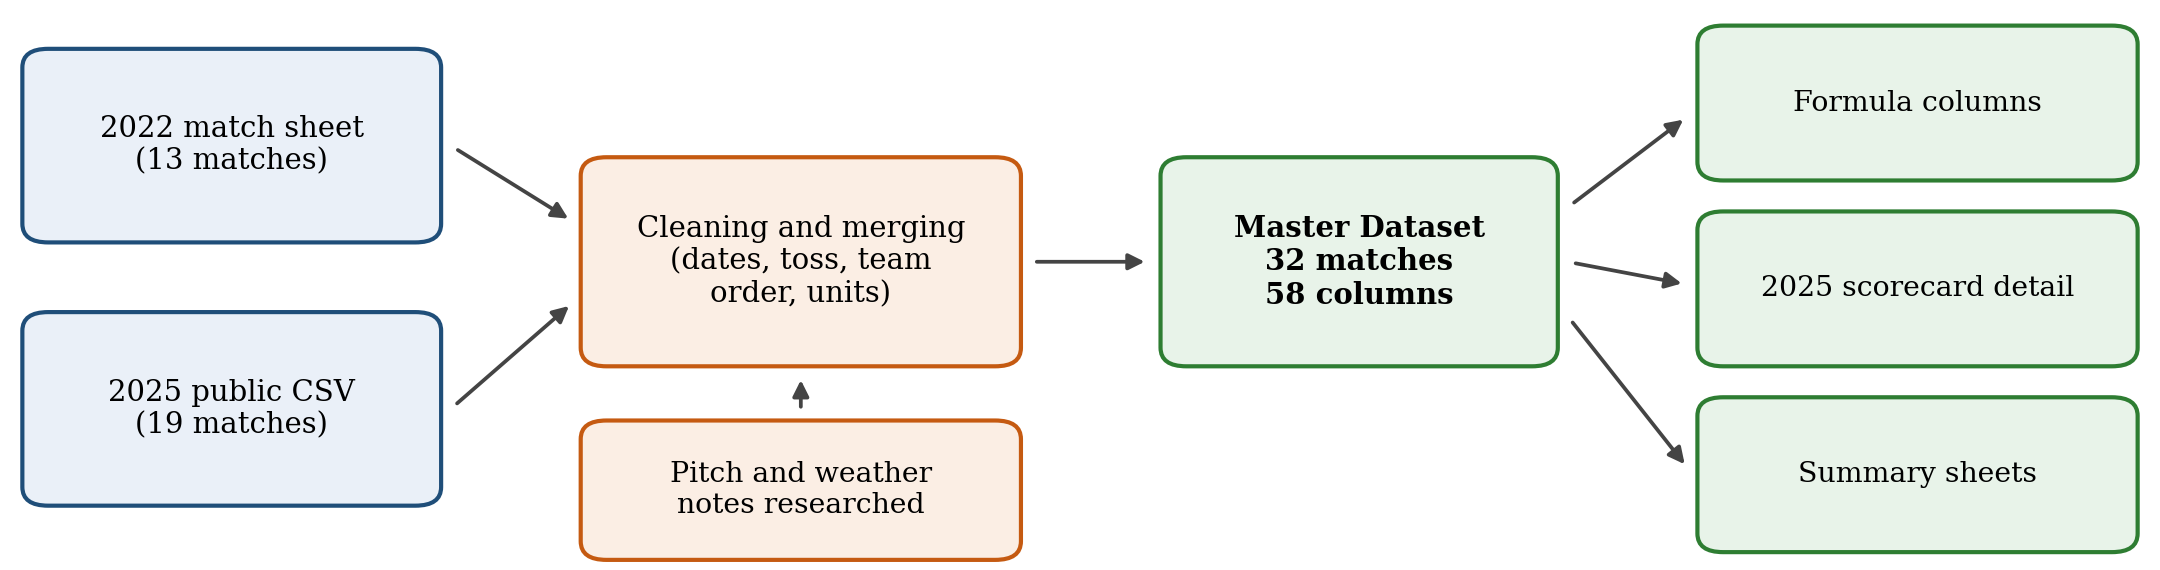
\includegraphics[width=0.9\textwidth]{fig_pipeline.png}
\caption{How the dataset was built. Two source files were cleaned and merged into one master table, extended with researched pitch and weather notes, and used to produce calculated fields, a detailed 2025 sheet and summary sheets.}
\label{fig:pipeline}
\end{figure*}

\runin{Scope.} Both tournaments were played in the T20 international format in the UAE. The 2022 edition had six teams and 13 matches, played at Dubai and Sharjah. The 2025 edition had eight teams, adding Oman and the UAE, and 19 matches, played at Dubai and Abu Dhabi. Each began with a group stage, followed by a Super Four stage and a final. Over the two years there were 18 group matches, 12 Super Four matches and 2 finals. Sri Lanka won in 2022 and India won in 2025.

\runin{Sources.} The 2022 rows were compiled by the authors, one row for each match. For 2025 we started from the dataset of Raza and Ali \cite{razadata}, which is shared under the CC BY 4.0 licence. Its authors collected the scorecards from ESPNcricinfo and checked them against information from the Asian Cricket Council \cite{razaarxiv,espn,acc}. We kept their match records, changed the layout, and made the corrections listed below. As the licence asks, we credit the original authors and state our changes.

For the 2025 pitch and weather notes we searched match by match. The weather condition came from the match page of a cricket website when one was available \cite{wisden}. Temperature, humidity and wind came from forecasts quoted in news previews, and the pitch descriptions came from previews, toss reports and expert reports \cite{news}. Each note carries a short text that names its source. We followed one rule, which was not to guess. For 2025, pitch notes exist for all 19 matches, weather condition for 17, temperature for 6, humidity for 2 and wind speed for 2. The temperature, humidity and wind figures are forecasts and not readings.

\runin{Errors fixed.} Joining sources turned up some small errors. Nine dates in the 2022 rows had the day and month swapped, so that 1 September appeared as 9 January. We rebuilt them and checked each one against the day of the week. The toss winner of India against Pakistan on 28 August 2022 was recorded as Pakistan, but match reports show that India won the toss and chose to field. In the 2025 file the first team column follows the schedule and not the batting order, so we reordered it. In our table \emph{Team~1 is always the side that batted first}. The 2025 file gave one start time for every match, but the organisers set most matches for 6:30 pm UAE time and one for 4 pm \cite{news}. We wrote the correct times together with Bangladesh time. We also replaced the title row with a plain header and used one spelling for each team and venue.

\runin{Fields added.} We added a match ID, series, stage, city and format, and 15 calculated fields written as spreadsheet formulas, so anyone can see how each value is worked out. One 2025 match, India against Sri Lanka in the Super Four stage, finished level at 202 runs each and was settled by a Super Over. We kept it and marked it clearly, so users can leave it out of win and loss analysis.
